\documentclass{standalone}
\usepackage{tikz}
\usetikzlibrary{patterns, positioning}


\begin{document}
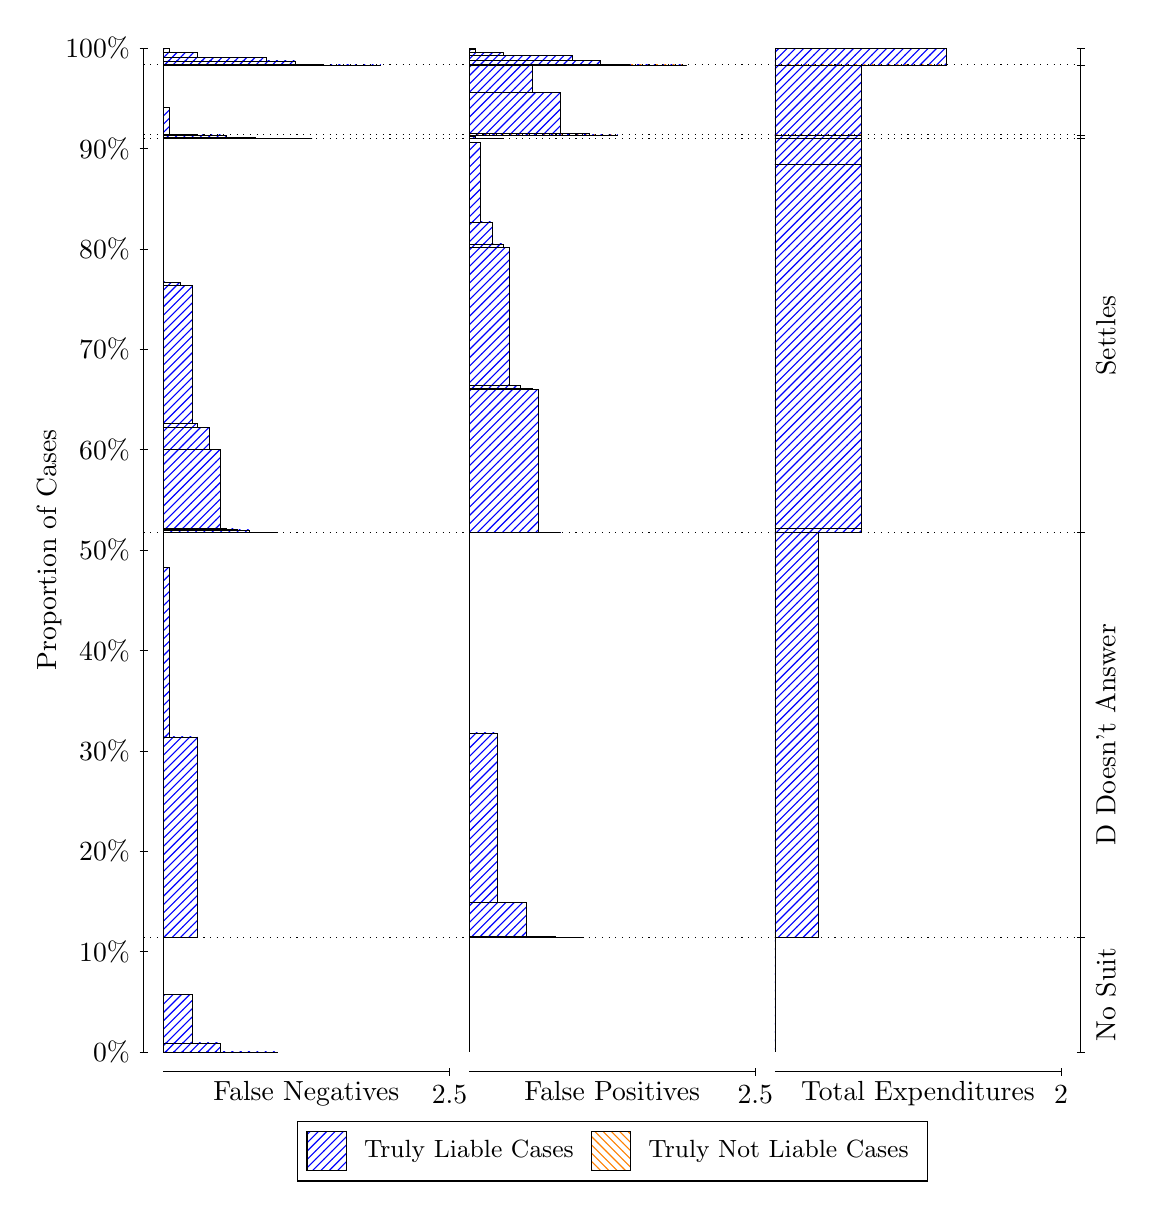
\begin{tikzpicture}
\draw[black, very thin] (1.5,1.75) -- (1.5,14.5);
\node[rotate=90, text=black, anchor=center] at (0.3, 8.125) {Proportion of Cases};
\draw[black, very thin] (1.45,1.75) -- (1.55,1.75);
\node[text=black, anchor=east] at (1.45, 1.75) {0\%};
\draw[black, very thin] (1.45,3.025) -- (1.55,3.025);
\node[text=black, anchor=east] at (1.45, 3.025) {10\%};
\draw[black, very thin] (1.45,4.3) -- (1.55,4.3);
\node[text=black, anchor=east] at (1.45, 4.3) {20\%};
\draw[black, very thin] (1.45,5.575) -- (1.55,5.575);
\node[text=black, anchor=east] at (1.45, 5.575) {30\%};
\draw[black, very thin] (1.45,6.85) -- (1.55,6.85);
\node[text=black, anchor=east] at (1.45, 6.85) {40\%};
\draw[black, very thin] (1.45,8.125) -- (1.55,8.125);
\node[text=black, anchor=east] at (1.45, 8.125) {50\%};
\draw[black, very thin] (1.45,9.4) -- (1.55,9.4);
\node[text=black, anchor=east] at (1.45, 9.4) {60\%};
\draw[black, very thin] (1.45,10.675) -- (1.55,10.675);
\node[text=black, anchor=east] at (1.45, 10.675) {70\%};
\draw[black, very thin] (1.45,11.95) -- (1.55,11.95);
\node[text=black, anchor=east] at (1.45, 11.95) {80\%};
\draw[black, very thin] (1.45,13.225) -- (1.55,13.225);
\node[text=black, anchor=east] at (1.45, 13.225) {90\%};
\draw[black, very thin] (1.45,14.5) -- (1.55,14.5);
\node[text=black, anchor=east] at (1.45, 14.5) {100\%};

\draw[black, very thin] (13.4,1.75) -- (13.4,14.5);
\draw[black, very thin] (13.35,1.75) -- (13.45,1.75);
\node[anchor=west] at (13.35, 1.75) {};
\draw[black, very thin] (13.35,3.2068) -- (13.45,3.2068);
\node[anchor=west] at (13.35, 3.2068) {};
\draw[black, very thin] (13.35,8.3478) -- (13.45,8.3478);
\node[anchor=west] at (13.35, 8.3478) {};
\draw[black, very thin] (13.35,13.351) -- (13.45,13.351);
\node[anchor=west] at (13.35, 13.351) {};
\draw[black, very thin] (13.35,13.398) -- (13.45,13.398);
\node[anchor=west] at (13.35, 13.398) {};
\draw[black, very thin] (13.35,14.286) -- (13.45,14.286);
\node[anchor=west] at (13.35, 14.286) {};
\draw[black, very thin] (13.35,14.5) -- (13.45,14.5);
\node[anchor=west] at (13.35, 14.5) {};

\draw[black, very thin, pattern color=blue, pattern=north east lines] (1.75,1.75) rectangle (3.2033,1.75);
\draw[black, very thin, pattern color=blue, pattern=north east lines] (1.75,1.75) rectangle (2.84,1.751);
\draw[black, very thin, pattern color=blue, pattern=north east lines] (1.75,1.751) rectangle (2.4767,1.8666);
\draw[black, very thin, pattern color=blue, pattern=north east lines] (1.75,1.8666) rectangle (2.1133,2.4794);
\draw[black, very thin, pattern color=orange, pattern=north west lines] (1.75,2.4794) rectangle (1.75,2.4794);
\draw[black, very thin, pattern color=blue, pattern=north east lines] (1.75,2.4794) rectangle (1.75,3.2068);
\draw[black, very thin, pattern color=blue, pattern=north east lines] (1.75,3.2068) rectangle (2.186,5.7527);
\draw[black, very thin, pattern color=blue, pattern=north east lines] (1.75,5.7527) rectangle (1.8227,7.9066);
\draw[black, very thin, pattern color=orange, pattern=north west lines] (1.75,7.9066) rectangle (1.75,7.9066);
\draw[black, very thin, pattern color=blue, pattern=north east lines] (1.75,7.9066) rectangle (1.75,8.3478);
\draw[black, very thin, pattern color=blue, pattern=north east lines] (1.75,8.3478) rectangle (3.2033,8.3478);
\draw[black, very thin, pattern color=blue, pattern=north east lines] (1.75,8.3478) rectangle (3.058,8.3478);
\draw[black, very thin, pattern color=blue, pattern=north east lines] (1.75,8.3478) rectangle (2.9127,8.3478);
\draw[black, very thin, pattern color=blue, pattern=north east lines] (1.75,8.3478) rectangle (2.84,8.3809);
\draw[black, very thin, pattern color=blue, pattern=north east lines] (1.75,8.3809) rectangle (2.6947,8.3942);
\draw[black, very thin, pattern color=blue, pattern=north east lines] (1.75,8.3942) rectangle (2.5493,8.3965);
\draw[black, very thin, pattern color=blue, pattern=north east lines] (1.75,8.3965) rectangle (2.4767,9.4066);
\draw[black, very thin, pattern color=blue, pattern=north east lines] (1.75,9.4066) rectangle (2.3313,9.6847);
\draw[black, very thin, pattern color=blue, pattern=north east lines] (1.75,9.6847) rectangle (2.186,9.7314);
\draw[black, very thin, pattern color=blue, pattern=north east lines] (1.75,9.7314) rectangle (2.1133,11.482);
\draw[black, very thin, pattern color=blue, pattern=north east lines] (1.75,11.482) rectangle (1.968,11.523);
\draw[black, very thin, pattern color=blue, pattern=north east lines] (1.75,11.523) rectangle (1.8227,11.53);
\draw[black, very thin, pattern color=orange, pattern=north west lines] (1.75,11.53) rectangle (1.75,11.53);
\draw[black, very thin, pattern color=blue, pattern=north east lines] (1.75,11.53) rectangle (1.75,13.351);
\draw[black, very thin, pattern color=blue, pattern=north east lines] (1.75,13.351) rectangle (3.6393,13.351);
\draw[black, very thin, pattern color=blue, pattern=north east lines] (1.75,13.351) rectangle (3.276,13.351);
\draw[black, very thin, pattern color=blue, pattern=north east lines] (1.75,13.351) rectangle (2.9127,13.367);
\draw[black, very thin, pattern color=blue, pattern=north east lines] (1.75,13.367) rectangle (2.5493,13.397);
\draw[black, very thin, pattern color=blue, pattern=north east lines] (1.75,13.397) rectangle (2.186,13.398);
\draw[black, very thin, pattern color=orange, pattern=north west lines] (1.75,13.398) rectangle (1.75,13.398);
\draw[black, very thin, pattern color=blue, pattern=north east lines] (1.75,13.398) rectangle (2.186,13.402);
\draw[black, very thin, pattern color=blue, pattern=north east lines] (1.75,13.402) rectangle (1.8227,13.745);
\draw[black, very thin, pattern color=orange, pattern=north west lines] (1.75,13.745) rectangle (1.75,13.745);
\draw[black, very thin, pattern color=blue, pattern=north east lines] (1.75,13.745) rectangle (1.75,14.286);
\draw[black, very thin, pattern color=blue, pattern=north east lines] (1.75,14.286) rectangle (4.5113,14.286);
\draw[black, very thin, pattern color=blue, pattern=north east lines] (1.75,14.286) rectangle (4.148,14.286);
\draw[black, very thin, pattern color=blue, pattern=north east lines] (1.75,14.286) rectangle (3.7847,14.289);
\draw[black, very thin, pattern color=blue, pattern=north east lines] (1.75,14.289) rectangle (3.4213,14.337);
\draw[black, very thin, pattern color=blue, pattern=north east lines] (1.75,14.337) rectangle (3.276,14.337);
\draw[black, very thin, pattern color=blue, pattern=north east lines] (1.75,14.337) rectangle (3.058,14.381);
\draw[black, very thin, pattern color=blue, pattern=north east lines] (1.75,14.381) rectangle (2.9127,14.381);
\draw[black, very thin, pattern color=blue, pattern=north east lines] (1.75,14.381) rectangle (2.6947,14.381);
\draw[black, very thin, pattern color=blue, pattern=north east lines] (1.75,14.381) rectangle (2.5493,14.383);
\draw[black, very thin, pattern color=blue, pattern=north east lines] (1.75,14.383) rectangle (2.3313,14.383);
\draw[black, very thin, pattern color=blue, pattern=north east lines] (1.75,14.383) rectangle (2.186,14.383);
\draw[black, very thin, pattern color=blue, pattern=north east lines] (1.75,14.383) rectangle (2.186,14.446);
\draw[black, very thin, pattern color=blue, pattern=north east lines] (1.75,14.446) rectangle (1.8227,14.446);
\draw[black, very thin, pattern color=blue, pattern=north east lines] (1.75,14.446) rectangle (1.8227,14.495);
\draw[black, very thin, pattern color=orange, pattern=north west lines] (1.75,14.495) rectangle (1.75,14.495);
\draw[black, very thin, pattern color=blue, pattern=north east lines] (1.75,14.495) rectangle (1.75,14.5);
\draw[black, very thin, pattern color=orange, pattern=north west lines] (5.6333,1.75) rectangle (5.6333,1.75);
\draw[black, very thin, pattern color=blue, pattern=north east lines] (5.6333,1.75) rectangle (5.6333,3.2068);
\draw[black, very thin, pattern color=orange, pattern=north west lines] (5.6333,3.2068) rectangle (7.0867,3.2068);
\draw[black, very thin, pattern color=blue, pattern=north east lines] (5.6333,3.2068) rectangle (7.0867,3.2069);
\draw[black, very thin, pattern color=blue, pattern=north east lines] (5.6333,3.2069) rectangle (6.7233,3.2193);
\draw[black, very thin, pattern color=blue, pattern=north east lines] (5.6333,3.2193) rectangle (6.36,3.648);
\draw[black, very thin, pattern color=blue, pattern=north east lines] (5.6333,3.648) rectangle (5.9967,5.8018);
\draw[black, very thin, pattern color=blue, pattern=north east lines] (5.6333,5.8018) rectangle (5.6333,8.3478);
\draw[black, very thin, pattern color=orange, pattern=north west lines] (5.6333,8.3478) rectangle (6.796,8.3478);
\draw[black, very thin, pattern color=blue, pattern=north east lines] (5.6333,8.3478) rectangle (6.796,8.3478);
\draw[black, very thin, pattern color=orange, pattern=north west lines] (5.6333,8.3478) rectangle (6.6507,8.3478);
\draw[black, very thin, pattern color=blue, pattern=north east lines] (5.6333,8.3478) rectangle (6.6507,8.3479);
\draw[black, very thin, pattern color=orange, pattern=north west lines] (5.6333,8.3479) rectangle (6.5053,8.3479);
\draw[black, very thin, pattern color=blue, pattern=north east lines] (5.6333,8.3479) rectangle (6.5053,10.168);
\draw[black, very thin, pattern color=blue, pattern=north east lines] (5.6333,10.168) rectangle (6.4327,10.175);
\draw[black, very thin, pattern color=blue, pattern=north east lines] (5.6333,10.175) rectangle (6.2873,10.217);
\draw[black, very thin, pattern color=blue, pattern=north east lines] (5.6333,10.217) rectangle (6.142,11.967);
\draw[black, very thin, pattern color=blue, pattern=north east lines] (5.6333,11.967) rectangle (6.0693,12.014);
\draw[black, very thin, pattern color=blue, pattern=north east lines] (5.6333,12.014) rectangle (5.924,12.292);
\draw[black, very thin, pattern color=blue, pattern=north east lines] (5.6333,12.292) rectangle (5.7787,13.302);
\draw[black, very thin, pattern color=blue, pattern=north east lines] (5.6333,13.302) rectangle (5.706,13.304);
\draw[black, very thin, pattern color=blue, pattern=north east lines] (5.6333,13.304) rectangle (5.6333,13.351);
\draw[black, very thin, pattern color=orange, pattern=north west lines] (5.6333,13.351) rectangle (6.0693,13.351);
\draw[black, very thin, pattern color=blue, pattern=north east lines] (5.6333,13.351) rectangle (6.0693,13.352);
\draw[black, very thin, pattern color=blue, pattern=north east lines] (5.6333,13.352) rectangle (5.706,13.381);
\draw[black, very thin, pattern color=blue, pattern=north east lines] (5.6333,13.381) rectangle (5.6333,13.398);
\draw[black, very thin, pattern color=orange, pattern=north west lines] (5.6333,13.398) rectangle (7.5227,13.398);
\draw[black, very thin, pattern color=blue, pattern=north east lines] (5.6333,13.398) rectangle (7.5227,13.398);
\draw[black, very thin, pattern color=blue, pattern=north east lines] (5.6333,13.398) rectangle (7.1593,13.412);
\draw[black, very thin, pattern color=blue, pattern=north east lines] (5.6333,13.412) rectangle (6.796,13.939);
\draw[black, very thin, pattern color=blue, pattern=north east lines] (5.6333,13.939) rectangle (6.4327,14.282);
\draw[black, very thin, pattern color=blue, pattern=north east lines] (5.6333,14.282) rectangle (6.0693,14.286);
\draw[black, very thin, pattern color=orange, pattern=north west lines] (5.6333,14.286) rectangle (8.3947,14.286);
\draw[black, very thin, pattern color=blue, pattern=north east lines] (5.6333,14.286) rectangle (8.3947,14.286);
\draw[black, very thin, pattern color=orange, pattern=north west lines] (5.6333,14.286) rectangle (8.0313,14.286);
\draw[black, very thin, pattern color=blue, pattern=north east lines] (5.6333,14.286) rectangle (8.0313,14.286);
\draw[black, very thin, pattern color=orange, pattern=north west lines] (5.6333,14.286) rectangle (7.668,14.286);
\draw[black, very thin, pattern color=blue, pattern=north east lines] (5.6333,14.286) rectangle (7.668,14.291);
\draw[black, very thin, pattern color=orange, pattern=north west lines] (5.6333,14.291) rectangle (7.3047,14.291);
\draw[black, very thin, pattern color=blue, pattern=north east lines] (5.6333,14.291) rectangle (7.3047,14.34);
\draw[black, very thin, pattern color=blue, pattern=north east lines] (5.6333,14.34) rectangle (6.9413,14.403);
\draw[black, very thin, pattern color=orange, pattern=north west lines] (5.6333,14.403) rectangle (6.796,14.403);
\draw[black, very thin, pattern color=blue, pattern=north east lines] (5.6333,14.403) rectangle (6.796,14.403);
\draw[black, very thin, pattern color=blue, pattern=north east lines] (5.6333,14.403) rectangle (6.578,14.405);
\draw[black, very thin, pattern color=orange, pattern=north west lines] (5.6333,14.405) rectangle (6.4327,14.405);
\draw[black, very thin, pattern color=blue, pattern=north east lines] (5.6333,14.405) rectangle (6.4327,14.405);
\draw[black, very thin, pattern color=blue, pattern=north east lines] (5.6333,14.405) rectangle (6.2147,14.405);
\draw[black, very thin, pattern color=blue, pattern=north east lines] (5.6333,14.405) rectangle (6.0693,14.449);
\draw[black, very thin, pattern color=orange, pattern=north west lines] (5.6333,14.449) rectangle (6.0693,14.449);
\draw[black, very thin, pattern color=blue, pattern=north east lines] (5.6333,14.449) rectangle (6.0693,14.449);
\draw[black, very thin, pattern color=blue, pattern=north east lines] (5.6333,14.449) rectangle (5.8513,14.449);
\draw[black, very thin, pattern color=blue, pattern=north east lines] (5.6333,14.449) rectangle (5.706,14.478);
\draw[black, very thin, pattern color=blue, pattern=north east lines] (5.6333,14.478) rectangle (5.706,14.497);
\draw[black, very thin, pattern color=blue, pattern=north east lines] (5.6333,14.497) rectangle (5.6333,14.5);
\draw[black, very thin, pattern color=orange, pattern=north west lines] (9.5167,1.75) rectangle (9.5167,1.75);
\draw[black, very thin, pattern color=blue, pattern=north east lines] (9.5167,1.75) rectangle (9.5167,3.2068);
\draw[black, very thin, pattern color=orange, pattern=north west lines] (9.5167,3.2068) rectangle (10.062,3.2068);
\draw[black, very thin, pattern color=blue, pattern=north east lines] (9.5167,3.2068) rectangle (10.062,8.3478);
\draw[black, very thin, pattern color=orange, pattern=north west lines] (9.5167,8.3478) rectangle (10.607,8.3478);
\draw[black, very thin, pattern color=blue, pattern=north east lines] (9.5167,8.3478) rectangle (10.607,8.4037);
\draw[black, very thin, pattern color=orange, pattern=north west lines] (9.5167,8.4037) rectangle (10.607,8.4037);
\draw[black, very thin, pattern color=blue, pattern=north east lines] (9.5167,8.4037) rectangle (10.607,13.018);
\draw[black, very thin, pattern color=orange, pattern=north west lines] (9.5167,13.018) rectangle (10.607,13.018);
\draw[black, very thin, pattern color=blue, pattern=north east lines] (9.5167,13.018) rectangle (10.607,13.351);
\draw[black, very thin, pattern color=orange, pattern=north west lines] (9.5167,13.351) rectangle (10.607,13.351);
\draw[black, very thin, pattern color=blue, pattern=north east lines] (9.5167,13.351) rectangle (10.607,13.398);
\draw[black, very thin, pattern color=orange, pattern=north west lines] (9.5167,13.398) rectangle (10.607,13.398);
\draw[black, very thin, pattern color=blue, pattern=north east lines] (9.5167,13.398) rectangle (10.607,14.286);
\draw[black, very thin, pattern color=orange, pattern=north west lines] (9.5167,14.286) rectangle (11.697,14.286);
\draw[black, very thin, pattern color=blue, pattern=north east lines] (9.5167,14.286) rectangle (11.697,14.5);
\draw[black, dotted] (1.5,3.2068) -- (13.4,3.2068);
\draw[black, dotted] (1.5,8.3478) -- (13.4,8.3478);
\draw[black, dotted] (1.5,13.351) -- (13.4,13.351);
\draw[black, dotted] (1.5,13.398) -- (13.4,13.398);
\draw[black, dotted] (1.5,14.286) -- (13.4,14.286);
\draw[black, very thin] (1.75,1.5) -- (5.3833,1.5);
\node[text=black, anchor=north] at (3.5667, 1.5) {False Negatives};
\draw[black, very thin] (5.3833,1.45) -- (5.3833,1.55);
\node[text=black, anchor=north] at (5.3833, 1.45) {2.5};

\draw[black, very thin] (5.6333,1.5) -- (9.2667,1.5);
\node[text=black, anchor=north] at (7.45, 1.5) {False Positives};
\draw[black, very thin] (9.2667,1.45) -- (9.2667,1.55);
\node[text=black, anchor=north] at (9.2667, 1.45) {2.5};

\draw[black, very thin] (9.5167,1.5) -- (13.15,1.5);
\node[text=black, anchor=north] at (11.333, 1.5) {Total Expenditures};
\draw[black, very thin] (13.15,1.45) -- (13.15,1.55);
\node[text=black, anchor=north] at (13.15, 1.45) {2};

\node[text=black, centered, rotate=90] at (13.72, 2.4784) {No Suit};
\node[text=black, centered, rotate=90] at (13.72, 5.7773) {D Doesn't Answer};
\node[text=black, centered, rotate=90] at (13.72, 10.849) {Settles};




\draw (7.449999999999999,1.5) node[draw=none] (baseCoordinate) {};
\begin{scope}[align=center]
        \matrix[scale=0.5, draw=black, below=0.5cm of baseCoordinate, nodes={draw}, column sep=0.1cm]{
            \node[rectangle, draw, minimum width=0.5cm, minimum height=0.5cm, pattern color=blue, pattern=north east lines] {}; &
            \node[draw=none, font=\small, text=black] (B) {Truly Liable Cases}; &
            \node[rectangle, draw, minimum width=0.5cm, minimum height=0.5cm, pattern color=orange, pattern=north west lines] {}; &
            \node[draw=none, font=\small, text=black] (B) {Truly Not Liable Cases}; \\
            };
\end{scope}

\end{tikzpicture}
\end{document}